\documentclass[a4paper,11pt]{article}
\input{/home/tof/Documents/Cozy/latex-include/preambule_lua.tex}
\newcommand{\showprof}{show them}  % comment this line if you don't want to see todo environment
\fancyhead[L]{TITRE}
\newdate{madate}{10}{09}{2020}
%\fancyhead[R]{\displaydate{madate}} %\today
%\fancyhead[R]{Seconde - SNT}
%\fancyhead[R]{Première - NSI}
\fancyhead[R]{Terminale - NSI}
\fancyfoot[L]{\vspace{1mm}Christophe Viroulaud}
\AtEndDocument{\label{lastpage}}
\fancyfoot[C]{\textbf{Page \thepage/\pageref{lastpage}}}
\fancyfoot[R]{\includegraphics[width=2cm,align=t]{/home/tof/Documents/Cozy/latex-include/cc.png}}

\begin{document}
\begin{center}
    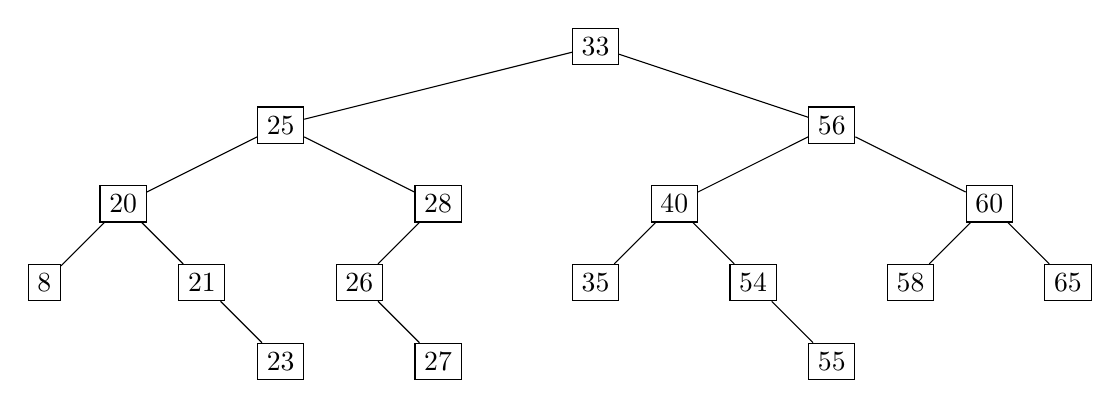
\begin{tikzpicture}
        \node[draw] (A) at (1,0) {33};
        \node[draw] (B) at (-3,-1) {25};
        \node[draw] (C) at (-5,-2) {20};
        \node[draw] (D) at (-1,-2) {28};
        \node[draw] (E) at (-6,-3) {8};
        \node[draw] (F) at (-4,-3) {21};
        \node[draw] (H) at (-2,-3) {26};
        \node[draw] (I) at (4,-1) {56};
        \node[draw] (J) at (2,-2) {40};
        \node[draw] (K) at (6,-2) {60};
        \node[draw] (M) at (1,-3) {35};
        \node[draw] (O) at (5,-3) {58};
        \node[draw] (P) at (7,-3) {65};
        \node[draw] (Q) at (-3,-4) {23};
        \node[draw] (R) at (-1,-4) {27};
        \node[draw] (S) at (3,-3) {54};
        \node[draw] (T) at (4,-4) {55};


        \draw (A) -- (B);
        \draw (C) -- (B);
        \draw (C) -- (E);
        \draw (C) -- (F);
        \draw (D) -- (B);
        \draw (D) -- (H);
        \draw (A) -- (I);
        \draw (J) -- (I);
        \draw (I) -- (K);
        \draw (J) -- (M);
        \draw (K) -- (O);
        \draw (K) -- (P);
        \draw (F) -- (Q);
        \draw (H) -- (R);
        \draw (J) -- (S);
        \draw (S) -- (T);
    \end{tikzpicture}
    \captionof{figure}{Activité 1}
    \label{arbre}
\end{center}
\end{document}